% بخش معماری پروژه MultiModal RAG
% این فایل جهت ادغام در main.tex طراحی شده است

\section{معماری سیستم}

این پروژه بر اساس الگوی معماری \lr{Clean Architecture} پیاده‌سازی شده است که امکان جداسازی مناسب نگرانی‌ها، مقیاس‌پذیری و نگهداری‌پذیری بالا را فراهم می‌آورد. انتخاب این معماری برای یک سیستم مبتنی بر مدل‌های زبانی بزرگ \lr{(LLM)} که نیازمند انعطاف‌پذیری بالا و قابلیت تست‌پذیری است، از اهمیت ویژه‌ای برخوردار است.

\begin{figure}[h]
    \centering
    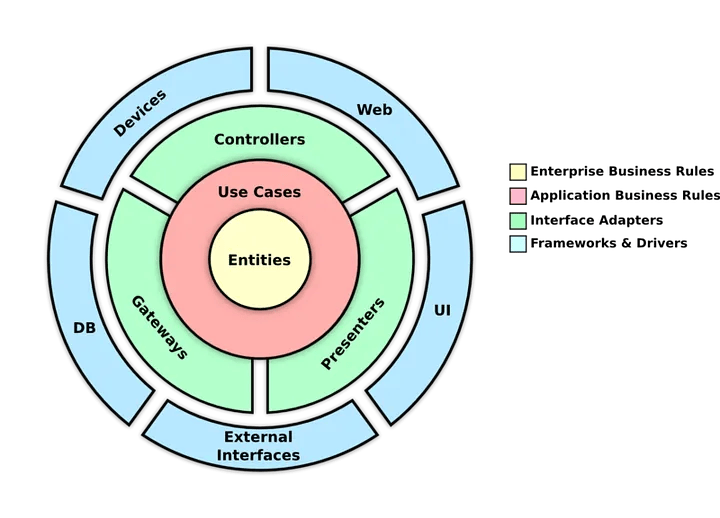
\includegraphics[width=0.8\textwidth]{clean_architecture.png}
    \caption{نمودار معماری \lr{Clean Architecture} و لایه‌های آن}
    \label{fig:clean_architecture}
\end{figure}

\noindent
شکل \ref{fig:clean_architecture} نمودار کلی معماری \lr{Clean} را نشان می‌دهد که در آن جهت وابستگی‌ها از بیرون به درون است و لایه‌های مرکزی از جزئیات پیاده‌سازی مستقل هستند.

\subsection{دلایل انتخاب معماری \lr{Clean}}

انتخاب معماری \lr{Clean} برای این پروژه بر اساس چندین معیار کلیدی صورت گرفته است:

\begin{itemize}    
    \item \textbf{قابلیت تست‌پذیری:} با جداسازی لایه‌های مختلف و استفاده از تزریق وابستگی \lr{(Dependency Injection)}، امکان نوشتن تست‌های واحد و یکپارچه با پوشش بالا میسر می‌شود.
    
    \item \textbf{انعطاف‌پذیری در تعویض ارائه‌دهندگان \lr{LLM}:} سیستم طراحی شده به گونه‌ای است که تغییر یا افزودن ارائه‌دهندگان مختلف \lr{LLM} (مانند \lr{OpenAI}، \lr{Cohere}، یا مدل‌های متن‌باز) بدون تغییر در منطق اصلی امکان‌پذیر است.
    
    \item \textbf{مقیاس‌پذیری:} ساختار لایه‌بندی شده امکان توسعه و گسترش سیستم را در آینده تسهیل می‌کند.
\end{itemize}

\subsection{لایه‌های معماری}

معماری این سیستم شامل چهار لایه اصلی است که هر کدام مسئولیت‌های مشخصی دارند و قانون وابستگی \lr{(Dependency Rule)} در آن‌ها رعایت می‌شود.

\subsubsection{لایه موجودیت‌ها \lr{(Entities)}}

این لایه، قلب سیستم را تشکیل می‌دهد و شامل \lr{enterprise business rules} است که مستقل از هرگونه جزئیات پیاده‌سازی خارجی هستند.

\noindent
\textbf{مسئولیت‌های این لایه:}
\begin{itemize}
    \item تعریف \lr{core data models} با استفاده از \lr{Pydantic}
    \item \lr{Data validation} و اعمال \lr{business rules}
    \item تضمین \lr{type-safety} و \lr{automatic serialization} داده‌ها
\end{itemize}

\noindent
به عنوان مثال، موجودیت \lr{\texttt{DocChunk}} در سیستم ما شامل قوانین کسب‌وکار زیر است:

\begin{itemize}
    \item \textbf{تولید شناسه یکتا:} هر \lr{chunk} باید دارای شناسه‌ای یکتا باشد که بر اساس \lr{\texttt{document\_id}} و \lr{index} تولید می‌شود: \lr{\texttt{\{document\_id\}\_chunk\_\{index\}}}
    
    \item \textbf{اعتبارسنجی بردار \lr{embedding}:} اگر بردار \lr{embedding} موجود باشد، باید از نوع \lr{\texttt{List[float]}} و غیر خالی باشد
    
    \item \textbf{حفظ \lr{metadata} اصلی:} تمام اطلاعات \lr{meta} شامل \lr{schema\_name}، \lr{version} و \lr{doc\_items} باید حفظ شوند
    
    \item \textbf{تبدیل فرمت:} موجودیت باید قابلیت تبدیل دوطرفه به فرمت \lr{Elasticsearch} و \lr{Docling} را داشته باشد
\end{itemize}

\noindent
این قوانین مستقل از جزئیات پیاده‌سازی \lr{database} یا \lr{search engine} تعریف شده‌اند و در صورت تغییر فناوری زیرساخت، دست‌نخورده باقی می‌مانند.


\subsubsection{لایه \lr{(Use Cases)}}

این لایه \lr{application business logic} را در بر می‌گیرد و \lr{workflow} بین \lr{entities} و \lr{interface adapters} را هماهنگ می‌کند.

\noindent
\textbf{مسئولیت‌های کلیدی:}
\begin{itemize}
    \item مدیریت جریان‌های کاری پیچیده با استفاده از \lr{LangGraph}
    \item پیاده‌سازی \lr{RAG (Retrieval-Augmented Generation) pipelines}
    \item تولید و مدیریت \lr{embeddings}
    \item هماهنگی با سرویس‌های خارجی از طریق \lr{interfaces}
\end{itemize}

\subsubsection{لایه آداپتورهای رابط \lr{(Interface Adapters)}}

این لایه وظیفه تبدیل داده‌ها بین موارد استفاده و دنیای خارج را بر عهده دارد.

\noindent
\textbf{اجزای این لایه شامل:}
\begin{itemize}
    \item \textbf{\lr{Controllers}:} مدیریت \lr{HTTP requests} و \lr{responses}
    \item \textbf{\lr{Presenters}:} قالب‌بندی داده‌ها برای رابط کاربری یا مصرف‌کنندگان \lr{API}
    \item \textbf{\lr{Gateways}:} رابط با سرویس‌های خارجی مانند \lr{databases}، \lr{vector stores} و \lr{third-party APIs}
\end{itemize}

\subsubsection{لایه فریم‌ورک‌ها و درایورها \lr{(Frameworks and Drivers)}}

بیرونی‌ترین لایه سیستم که شامل جزئیات پیاده‌سازی ابزارها و فریم‌ورک‌های خارجی است.

\noindent
\textbf{مثال‌های موجود در این لایه:}
\begin{itemize}
    \item \lr{Web frameworks} (\lr{FastAPI}، \lr{Flask})
    \item \lr{LLM providers} (\lr{OpenAI}، \lr{Cohere}، \lr{open-source models})
    \item \lr{Databases} و \lr{vector stores} (\lr{Elasticsearch}، \lr{Redis}، \lr{Pinecone})
\end{itemize}

\subsection{اصول طراحی}

\subsubsection{قانون وابستگی \lr{(Dependency Rule)}}

در این معماری، وابستگی‌ها همواره از لایه‌های بیرونی به سمت لایه‌های درونی هستند. این بدان معناست که:

\begin{equation}
\text{\lr{Frameworks/Drivers}} \rightarrow \text{\lr{Interface Adapters}} \rightarrow \text{\lr{Use Cases}} \rightarrow \text{\lr{Entities}}
\end{equation}

\noindent
لایه‌های درونی هیچ‌گونه اطلاعی از لایه‌های بیرونی ندارند و این استقلال امکان تغییر پیاده‌سازی‌های خارجی را بدون تأثیر بر هسته سیستم فراهم می‌آورد.

\subsubsection{اصل وارونگی وابستگی \lr{(Dependency Inversion Principle)}}

برای حفظ قانون وابستگی، از \lr{interfaces} و کلاس‌های انتزاعی استفاده می‌شود. به این ترتیب:

\begin{itemize}
    \item \lr{Interfaces} در لایه‌های هسته (\lr{Use Cases}) تعریف می‌شوند
    \item پیاده‌سازی‌های واقعی در لایه‌های بیرونی (\lr{Interface Adapters} یا \lr{Frameworks}) قرار می‌گیرند
    \item لایه‌های سطح بالا به انتزاع وابسته‌اند، نه به پیاده‌سازی‌های خاص
\end{itemize}


\noindent

\textbf{مثال کاربردی:} در سیستم ما، \lr{use case}ای به نام \lr{agentic\_rag} ماژولی از نوع \lr{EmbeddingServiceInterface} دریافت می‌کند. این \lr{use case} توابعی مانند \lr{embed\_single} را فراخوانی می‌کند، بدون آنکه بداند پیاده‌سازی واقعی از چه ارائه‌دهنده‌ای استفاده می‌کند (مانند \lr{OpenAI}، \lr{Google GenAI}، \lr{Azure}، یا مدل‌های متن‌باز). این امر به این دلیل امکان‌پذیر است که:

\begin{itemize}
    \item \lr{Use case} تنها به \lr{contract} تعریف شده در \lr{interface} وابسته است
    \item تعویض ارائه‌دهنده \lr{embedding} بدون تغییر در منطق کسب‌وکار به راحتی امکان‌پذیر است
\end{itemize}

\subsection{سیستم \lr{Dependency Injection}}

برای مدیریت وابستگی‌ها و پیکربندی سیستم، از کتابخانه \lr{\texttt{dependency-injector}} استفاده شده است. این سیستم مزایای زیر را فراهم می‌آورد:

\subsubsection{مزایای \lr{Dependency Injection}}

\begin{itemize}
    \item \textbf{\lr{Centralized configuration}:} تمام تنظیمات و وابستگی‌ها در یک \lr{container} مرکزی مدیریت می‌شوند
    \item \textbf{تسهیل تست:} امکان جایگزینی وابستگی‌های واقعی با \lr{mocks} برای تست‌نویسی
    \item \textbf{مدیریت \lr{singleton}:} کنترل \lr{lifecycle} منابع گران‌قیمت مانند \lr{database connections}
    \item \textbf{انعطاف‌پذیری:} تغییر \lr{configuration} در \lr{runtime} بدون تغییر کد
\end{itemize}

\noindent
\textbf{انواع \lr{providers} در کتابخانه \lr{dependency-injector}:}
\begin{itemize}
    \item \textbf{\lr{Factory}:} برای ایجاد نمونه جدید در هر بار استفاده. این نوع \lr{provider} هر بار که درخواست می‌شود، یک \lr{instance} جدید از کلاس مورد نظر ایجاد می‌کند. برای اشیائی مناسب است که \lr{stateless} هستند یا هر بار نیاز به تنظیمات تازه دارند.
    
    \item \textbf{\lr{Singleton}:} برای نگهداری یک نمونه واحد در طول عمر برنامه. این \lr{provider} فقط یک بار شیء را می‌سازد و در تمام درخواست‌های بعدی همان نمونه را بازمی‌گرداند. برای منابع گران‌قیمت مانند اتصالات \lr{database}، \lr{HTTP clients} یا \lr{configuration objects} مفید است.
    
    \item \textbf{\lr{Resource}:} برای مدیریت چرخه حیات اشیاء پیچیده که نیاز به راه‌اندازی و پاکسازی دارند. این \lr{provider} قابلیت‌های \lr{lifecycle management} مانند \lr{initialization}، \lr{cleanup} و مدیریت منابع سیستمی را فراهم می‌آورد. برای سرویس‌هایی که نیاز به \lr{graceful shutdown} دارند، ایده‌آل است.
    
    \item \textbf{\lr{Configuration}:} برای مدیریت و تزریق مقادیر پیکربندی مانند \lr{environment variables}، تنظیمات \lr{API}، یا پارامترهای سیستم. این \lr{provider} امکان خواندن مقادیر از فایل‌های \lr{config}، متغیرهای محیطی یا منابع خارجی را فراهم می‌آورد و آن‌ها را در سراسر سیستم در دسترس قرار می‌دهد.
\end{itemize}

\subsection{یکپارچگی با فریم‌ورک‌های \lr{LLM}}

یکی از چالش‌های اصلی این پروژه، یکپارچگی با فریم‌ورک‌های مختلف \lr{LLM} بوده است. معماری طراحی شده این امکان را فراهم می‌آورد که:

\begin{itemize}
    \item از چندین ارائه‌دهنده \lr{LLM} به صورت همزمان استفاده شود
    \item جریان‌های کاری پیچیده با \lr{LangGraph} مدیریت شوند
    \item عملیات \lr{RAG} به صورت ماژولار پیاده‌سازی شوند
    \item تغییر یا ارتقای فریم‌ورک‌ها بدون تغییر منطق اصلی امکان‌پذیر باشد
\end{itemize}

\subsection{استفاده از \lr{Pydantic}}

در لایه موجودیت‌ها، از کتابخانه \lr{Pydantic} برای تعریف \lr{data models} استفاده شده است. این انتخاب به دلایل زیر صورت گرفته است:

\begin{itemize}
    \item \textbf{\lr{Automatic validation}:} داده‌ها به صورت خودکار در زمان ایجاد \lr{object} اعتبارسنجی می‌شوند
    \item \textbf{\lr{Type Safety}:} تضمین صحت \lr{data types} در زمان توسعه
    \item \textbf{\lr{Serialization}:} تبدیل خودکار به \lr{JSON} و سایر فرمت ها
    \item \textbf{\lr{Automatic documentation}:} تولید \lr{schema} برای \lr{API}ها
\end{itemize}

\subsection{مدیریت \lr{Error} و \lr{Logging}}

سیستم دارای یک لایه یکپارچه برای \lr{error handling} و \lr{logging} است که:

\begin{itemize}
    \item از \lr{multi-level logging} پشتیبانی می‌کند
    \item خطاها را به صورت ساختاریافته ثبت می‌کند
    \item امکان \lr{request tracing} را فراهم می‌آورد
    \item با سیستم‌های \lr{monitoring} خارجی قابل یکپارچگی است
\end{itemize}

\noindent
به عنوان مثال، میتوان از \lr{Prometheus} برای جمع‌آوری متریک ها و از \lr{Grafana} برای \lr{visualization} استفاده کرد تا به اهداف زیر رسید:

\begin{itemize}
    \item \textbf{\lr{Metrics Collection}:} \lr{Response times}، تعداد درخواست‌ها، نرخ خطا، و استفاده از منابع
    \item \textbf{\lr{Health Checks}:} بررسی وضعیت سرویس‌های \lr{LLM}، \lr{database connections}، و \lr{vector stores}
    \item \textbf{\lr{Alerting}:} اطلاع‌رسانی خودکار در صورت بروز مشکل از طریق \lr{Slack} یا \lr{Email}
\end{itemize}

\noindent
سیستم \lr{logging} پیاده‌سازی شده در این پروژه، از قابلیت \lr{automatic rotation} و مدیریت \lr{log levels} مختلف برخوردار است. شکل \ref{fig:logging_example} نمونه‌ای از خروجی سیستم \lr{logging} را نشان می‌دهد که شامل \lr{timestamp}، نام \lr{module}، \lr{log level}، و \lr{message} مربوطه است.

\begin{figure}[h]
    \centering
    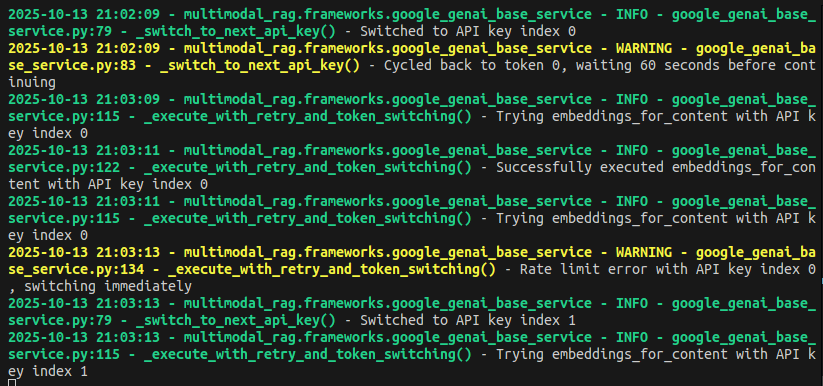
\includegraphics[width=\textwidth]{logging_example.png}
    \caption{نمونه \lr{output} سیستم \lr{logging}}
    \label{fig:logging_example}
\end{figure}

\subsection{نتیجه‌گیری معماری}

معماری \lr{Clean} برای این پروژه \lr{MultiModal RAG}، بستری مناسب برای توسعه یک سیستم \lr{scalable}، \lr{maintainable} و \lr{flexible} فراهم آورده است. جداسازی واضح لایه‌ها، استفاده از \lr{dependency injection}، و رعایت اصول \lr{SOLID}، امکان توسعه پایدار و با کیفیت این سیستم را در بلندمدت تضمین می‌کند. این رویکرد معماری به‌ویژه برای سیستم‌های مبتنی بر \lr{LLM} که نیازمند \lr{flexibility} بالا در تعویض \lr{providers} و \lr{models} هستند، مناسب است.
